\section{Design}
\label{sec:desgin}
\lhead{\thesection \space Design}

TODO Lucas

\subsection{Functionality}
\label{ssec:functionality}

Since the application is supposed to offer a certain set of features to the user, it needed to be defined what kind of functionality was necessary to ensure that a user could interact with all the features the application has to offer. This section details this set of features and their functionality.
\newline
Each functionality is described using a set of diagrams, such as state machine or activity diagrams. A visual representation can also be found in \textit{\ref{ssec:visual_design} \nameref{ssec:visual_design}}.

\subsubsection{Creating a new Poll}
\label{sssec:creating_a_new_poll}

Since the \textit{Vote4Fun} extension is about creating a poll and letting users vote on it, the actual creation of such a poll is of course an important and arguably biggest piece of functionality. The polls are divided into two categories, which are a regular and an "on-the-fly" poll.
\newline
The regular poll is created for one specific team, as shown in Figure \ref{fig:state_machine_diagram_create_poll}. The owner of the poll simply picks a team and is able to add guests to the poll afterwards. Each guest is checked for validity, in this case whether the entered email address representing the guest is an active user of \textit{Connected.Football}. This can be repeated for multiple users. An "on-the-fly" poll does not require a team, but rather a set of email addresses, which do not need to be registered on \textit{Connected.Football}. Once the owner has entered the email addresses, a temporary team is created (see \textit{\ref{sssec:creating_temp_team} \nameref{sssec:creating_temp_team}}).
\newline
In both cases, the poll has a set of users. Once the owner enters information regarding the deadline and exercises to be voted upon, the poll itself is created. This is followed by notifications being sent to all users participating in the poll.

\begin{figure}[H]
    \begin{center}
        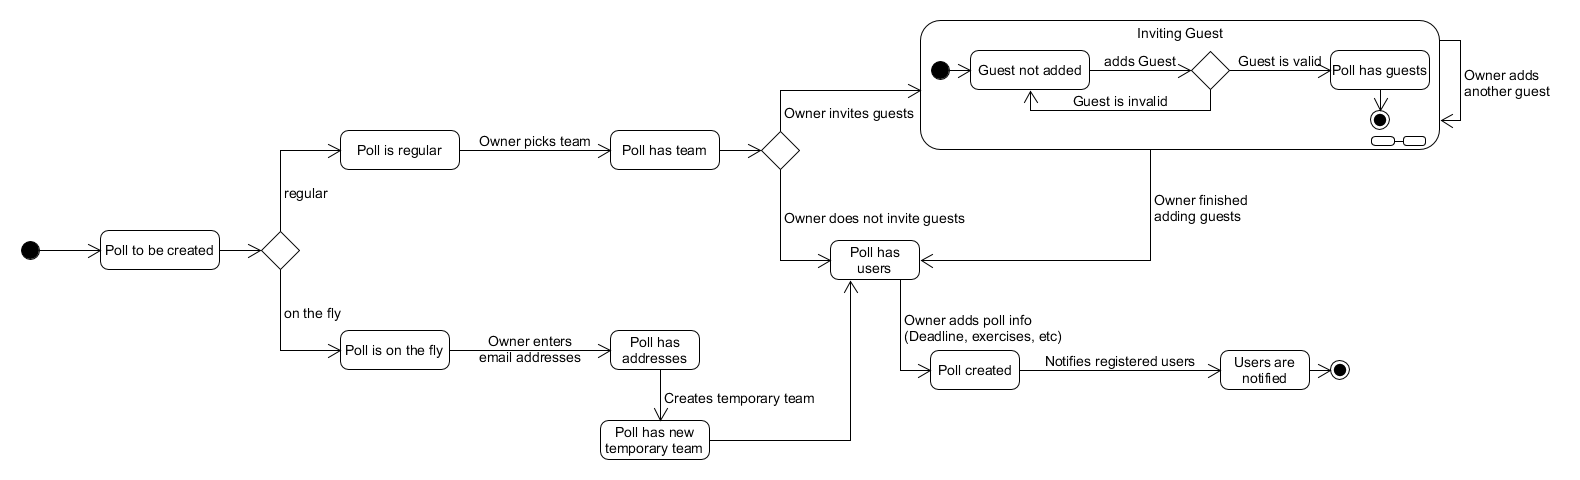
\includegraphics[width=1\textwidth]{images/diagrams/state_machine_diagrams/StateDiagram_CreatePoll.png}
        \caption{State Machine Diagram Create Poll}
        \label{fig:state_machine_diagram_create_poll}
    \end{center}
\end{figure}

TODO Lucas Describe Activity Diagram Create Exercise Poll

\begin{figure}[H]
    \begin{center}
        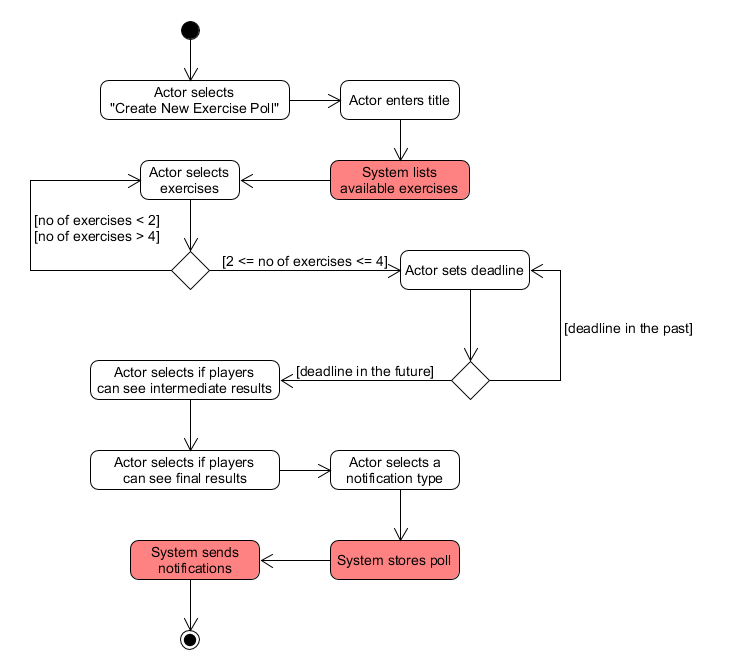
\includegraphics[width=0.8\textwidth]{images/diagrams/activity_diagrams/ActivityDiagram_CreateExercisePoll.png}
        \caption{Activity Diagram Create Poll}
        \label{fig:activity_diagram_create_poll}
    \end{center}
\end{figure}

\subsubsection{Creating a Temporary Team}
\label{sssec:creating_temp_team}

As mentioned in \textit{\ref{sssec:creating_a_new_poll} \nameref{sssec:creating_a_new_poll}}, when an "on-the-fly" poll is created, a new temporary team is created as well. This team consists of people that may or may not be registered with the \textit{Connected.Football} platform. Unfortunately, this functionality was not implemented in time, but since it is required for Epic 3 (see \textit{\ref{sssec:epic3} \nameref{sssec:epic3}}, it is mentioned for the sake of completeness and for future reference.
\newline
As seen in Figure \ref{fig:state_machine_diagram_create_temp_team}, the process starts with the owner of the poll entering an email address representing the person they want to add to the temporary team. If the email is not properly formatted, the entry is discarded. If the format is correct, the address is stored and the owner can either add another email address or they can continue.
\newline
The \textit{Connected.Football} platform than checks for every entered email address whether a user with the same address is already registered. If that is the case, the reference to the already existing user is stored in the temporary team and the user is sent a push notification. If not, the platform creates a callback and sends an invitation to the email address. This invitation was supposed to be handled by \textit{Firebase}, which provides functionality for such an on-boarding process. If the user follows this invitation, the callback is triggered, which stores the new user in the temporary team, once they have completed their registration.

\begin{figure}[H]
    \begin{center}
        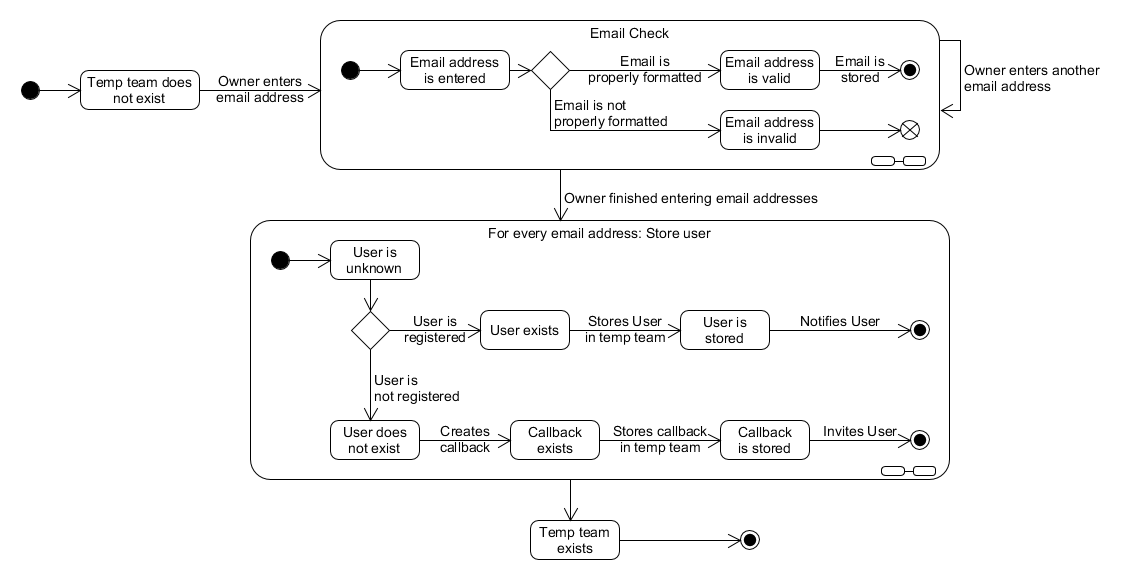
\includegraphics[width=1\textwidth]{images/diagrams/state_machine_diagrams/StateDiagram_CreateTempTeam.png}
        \caption{State Machine Diagram Create Temporary Team}
        \label{fig:state_machine_diagram_create_temp_team}
    \end{center}
\end{figure}

\subsubsection{Voting on an Exercise Poll}
\label{sssec:voting_on_exercise_poll}

TODO Lucas Describe Activity Diagram Vote on Poll

\begin{figure}[H]
    \begin{center}
        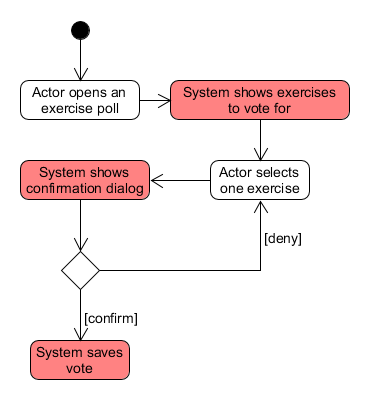
\includegraphics[width=0.5\textwidth]{images/diagrams/activity_diagrams/ActivityDiagram_VoteOnExercisePoll.png}
        \caption{Activity Diagram Vote on Poll}
        \label{fig:activity_diagram_vote_on_poll}
    \end{center}
\end{figure}

\subsubsection{Entering a Promotion Code}
\label{sssec:entering_promotion_code}

TODO Lucas Describe Activity Diagram Enter Promotion Code

\begin{figure}[H]
    \begin{center}
        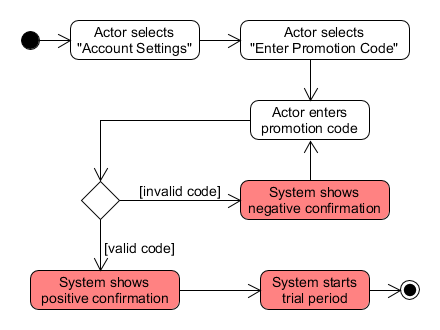
\includegraphics[width=0.6\textwidth]{images/diagrams/activity_diagrams/ActivityDiagram_EnterPromotionCode.png}
        \caption{Activity Diagram Enter Promotion Code}
        \label{fig:activity_diagram_enter_promotion_code}
    \end{center}
\end{figure}

\subsection{Visual Design}
\label{ssec:visual_design}

TODO Lucas, TODO Marco

\subsection{\textit{Vote4Fun} Object Definition}
\label{ssec:vote4fun_object_definition}

TODO Marco

\subsection{Component Structure}
\label{ssec:component_structure}

TODO Sebastian